\chapter{Scenarios Analysis}

% TODO:
% - intro
% - overview of the results in the categories
% - two dimensions across time and across category
% - divide in categories
% - for each category analyze the graph, over time
%     1) then we can look at the metrics averaged (over time)
%         - TABLE + comment on table:
%             - differences among categories on average 
%             - page rank median
%             - bar chart categories by degree?
%     2) time series of some metric in some categories 

% -specific examples - Food & Gas: 
%     1) graph metrics: 
%         - over time
%         - power law over time
%     2) node properties:
%         - compared on average tra i nodi
%         - time series of relevant node's + pr
%     3) communities:
%         - grafico schschschschscsch (x2)
%         - plot confronto sbm vs louv 
%             --> fai vedere in cosa sono diversi (perchè le communities rappresentano cose diverse)
%             --> confronto modularities
%         - plot tanti^n plot


The core idea of my research is to study methods of network theory with the goal of applying them to the constructed dataset of import/export exchanges among countries. The purpose of this chapter is to show the results obtained from the analysis of the total network and of more sectorial networks, and to comment on the metrics and visualization that have been produced, in order to demonstrate the insights one would be able to obtain by applying the methodology proposed in previous chapters. Therefore, I use the cleaned, normalized data from Chapter \ref{ch:2data} and analyze them using the approaches described in Chapter \ref{ch:3methods}.
% Maybe insert some general features of the dataset, either here or on ch 2
The dataset of trade exchanges provides us with two dimensions along which one can conduct the analysis. The first one is the product category. In fact, thanks to the standardized nomenclature adopted by most countries, we can identify the relevant markets [ESEMPIO CIBO, ALTRE COSE] easily, and zoom in, from the general view of the total exchanges, to the structure of a specific group of products, in which perhaps some countries may emerge as more central, or we can spot more easily possible dependencies of one country from another. The way in which the nomenclature is constructed allows to possibly choose different levels of granularity of the data. As shown in Section \ref{sec:nomandusd}, the more comprehensive collections are indicated by a two-digit code, while moving to three or four-digit codes characterizes more specific sub-categories of products. 
The second dimension of interest is time: the reported imports and exports are aggregated annually, and therefore we have information about the state of the world trade network in each year, from 2001 until 2020. We can see how the graph evolved, how its metrics changed over time, and we can have a general understanding of the complex net of interactions among countries, and of the competitiveness of the market.

What I have done is to divide the dataset according to the two-digit categories, focusing only on the two-digit code, construct a graph of each category in every available year, and then compute metrics and run algorithms to uncover patterns in the network structures.
Let us have a look at Table \ref{tab:catmetrics}, in which I reported the main graph and node metrics for each category.

\begin{landscape}
\begin{table}
    \begin{tabular}{llrrrrrr}
\toprule
Product Code & Product Categories & Mean Num. Edges & Mean Sum Weights & Mean Degree & Mean Weighted Degree & Mean Density & Mean Clustering Coef. \\
\midrule
 TO & Total & 17575.050 & 942947843.701 & 148.313 & 3978682.885 & 0.314 & 0.648 \\
 19 & Coke and refined petroleum products & 4721.800 & 167109502.967 & 39.846 & 705103.388 & 0.084 & 0.501 \\
 30 & Other transport equipment & 6483.400 & 110930370.321 & 54.712 & 468060.634 & 0.116 & 0.573 \\
 26 & Computer, electronic and optical products & 11274.950 & 96660694.247 & 95.147 & 407851.031 & 0.202 & 0.623 \\
 28 & Machinery and equipment n.e.c. & 10868.350 & 54938507.830 & 91.716 & 231808.050 & 0.194 & 0.611 \\
 29 & Motor vehicles, trailers and semi-trailers & 8175.600 & 51056661.847 & 68.992 & 215428.953 & 0.146 & 0.571 \\
 20 & Chemicals and chemical products & 10120.850 & 48331862.230 & 85.408 & 203931.908 & 0.181 & 0.607 \\
 10 & Food products & 10335.950 & 46061450.323 & 87.223 & 194352.111 & 0.185 & 0.600 \\
 24 & Basic metals & 7263.050 & 38514452.032 & 61.292 & 162508.236 & 0.130 & 0.580 \\
 27 & Electrical equipment & 10454.500 & 33900343.502 & 88.224 & 143039.424 & 0.187 & 0.613 \\
 06 & Crude petroleum and natural gas & 1141.700 & 26312732.619 & 9.635 & 111024.188 & 0.020 & 0.189 \\
 25 & Fabricated metal products, except machinery and equipment & 9896.300 & 25927827.433 & 83.513 & 109400.116 & 0.177 & 0.602 \\
 35 & Electricity, gas, steam and air conditioning & 337.750 & 24201517.246 & 2.850 & 102116.107 & 0.006 & 0.092 \\
 32 & Other manufactured goods & 10164.500 & 23740467.914 & 85.776 & 100170.751 & 0.182 & 0.621 \\
 21 & Basic pharmaceutical products and pharmaceutical preparations & 6758.000 & 23043166.709 & 57.030 & 97228.552 & 0.121 & 0.563 \\
 22 & Rubber and plastic products & 9687.900 & 17939948.214 & 81.754 & 75695.984 & 0.173 & 0.594 \\
 XX & Unknown & 5771.050 & 17629317.147 & 48.701 & 74385.304 & 0.103 & 0.453 \\
 14 & Wearing apparel & 10303.300 & 17521060.729 & 86.948 & 73928.526 & 0.184 & 0.600 \\
 01 & Products of agriculture, hunting and related services & 9014.200 & 12713697.276 & 76.069 & 53644.292 & 0.161 & 0.561 \\
 23 & Other non-metallic mineral products & 8216.450 & 12329042.801 & 69.337 & 52021.278 & 0.147 & 0.581 \\
 11 & Beverages & 6203.250 & 10641519.052 & 52.348 & 44900.924 & 0.111 & 0.558 \\
 17 & Paper and paper products & 7544.350 & 10490896.358 & 63.665 & 44265.385 & 0.135 & 0.581 \\
 13 & Textiles & 8974.000 & 9972507.572 & 75.730 & 42078.091 & 0.160 & 0.588 \\
 15 & Leather and related products & 8229.500 & 7924403.622 & 69.447 & 33436.302 & 0.147 & 0.581 \\
 31 & Furniture & 7016.850 & 7669984.697 & 59.214 & 32362.805 & 0.125 & 0.560 \\
 16 & Wood and of products of wood and cork, except furniture; articles of straw and plaiting materials & 7022.050 & 6020516.928 & 59.258 & 25403.025 & 0.126 & 0.567 \\
 MM & Adjustments ( broken down at chapter level only) & 501.450 & 5328187.945 & 4.232 & 22481.806 & 0.009 & 0.089 \\
 12 & Tobacco products & 3032.000 & 4970535.504 & 25.586 & 20972.724 & 0.054 & 0.399 \\
 38 & Waste collection, treatment and disposal services; materials recovery services & 4704.000 & 4814771.324 & 39.696 & 20315.491 & 0.084 & 0.524 \\
 SS & Confidential data & 1917.750 & 4307264.746 & 16.184 & 18174.113 & 0.034 & 0.707 \\
 58 & Publishing services & 8320.250 & 3798567.540 & 70.213 & 16027.711 & 0.149 & 0.583 \\
 08 & Other mining and quarrying products & 4947.250 & 3359659.380 & 41.749 & 14175.778 & 0.088 & 0.520 \\
 07 & Metal ores & 1870.650 & 2429029.316 & 15.786 & 10249.069 & 0.033 & 0.328 \\
 EE & Selections of goods & 399.500 & 1751829.756 & 3.371 & 7391.687 & 0.007 & 0.000 \\
 05 & Coal and lignite & 905.050 & 1747408.161 & 7.638 & 7373.030 & 0.016 & 0.197 \\
 90 & Creative, arts and entertainment services & 3575.550 & 1384069.138 & 30.173 & 5839.954 & 0.064 & 0.447 \\
 59 & Motion picture, video and television programme production services, sound recording and music publishing & 4249.350 & 1236208.370 & 35.859 & 5216.069 & 0.076 & 0.519 \\
 03 & Fish and other fishing products; aquaculture products; support services to fishing & 2354.100 & 1079356.697 & 19.866 & 4554.248 & 0.042 & 0.441 \\
 BB & Articles declared as supplies or services for ships and aircrafts  & 717.950 & 967973.730 & 6.059 & 4084.277 & 0.013 & 0.203 \\
 RR & Returned goods & 914.100 & 931754.965 & 7.714 & 3931.456 & 0.016 & 0.644 \\
 91 & Library, archive, museum and other cultural services & 2167.100 & 779059.619 & 18.288 & 3287.171 & 0.039 & 0.462 \\
 02 & Products of forestry, logging and related services & 3592.300 & 629720.502 & 30.315 & 2657.049 & 0.064 & 0.417 \\
 VV & Parts for motor vehicles & 269.812 & 452194.449 & 2.277 & 1907.993 & 0.005 & 0.096 \\
 II & Components of complete industrial plant & 218.600 & 349448.273 & 1.845 & 1474.465 & 0.004 & 0.107 \\
 YY & Adjustments (not broken down at chapter level) & 289.550 & 345893.271 & 2.443 & 1459.465 & 0.005 & 0.100 \\
 CC & Temporary corrections due to erroneous codes & 735.600 & 260218.547 & 6.208 & 1097.969 & 0.013 & 0.310 \\
 74 & Other professional, scientific and technical services & 1008.550 & 192669.026 & 8.511 & 812.949 & 0.018 & 0.258 \\
 AA & Intra-EU trade involving transactions falling below the simplification threshold & 472.350 & 180721.329 & 3.986 & 762.537 & 0.008 & 0.141 \\
 PP & Goods transported by post & 403.150 & 172805.626 & 3.402 & 729.138 & 0.007 & 0.129 \\
 WW & Parts for aircrafts & 140.312 & 82302.400 & 1.184 & 347.268 & 0.003 & 0.043 \\
 18 & Printing and reproduction services of recorded media & 1553.900 & 71517.232 & 13.113 & 301.760 & 0.028 & 0.337 \\
 FF & Articles declared as supplies or services for offshore installations & 107.562 & 15482.768 & 0.908 & 65.328 & 0.002 & 0.045 \\
 UU & Unknown (to be checked) & 271.000 & 15434.795 & 2.287 & 65.126 & 0.005 & 0.000 \\
 71 & Architectural and engineering services; technical testing and analysis services & 1186.350 & 12419.911 & 10.011 & 52.405 & 0.021 & 0.276 \\
 TT & Foodstuff, drinks and tobacco & 157.250 & 11327.795 & 1.327 & 47.797 & 0.003 & 0.087 \\
 96 & Other personal services & 230.300 & 2510.194 & 1.943 & 10.592 & 0.004 & 0.055 \\
 37 & Sewerage services; sewage sludge & 100.895 & 597.688 & 0.851 & 2.522 & 0.002 & 0.026 \\
\bottomrule
\end{tabular}

    \caption{Category metrics}
    \label{tab:catmetrics}
\end{table}

\end{landscape}

The table is obtained by taking the graphs of each category, computing the metrics and averaging across years and nodes, while keeping fixed the number of countries under consideration, i.e. 237 territories.
It is sorted according to the Average Sum of Weights, which is an indicator of the size of that trading market over the last 20 years. The first row refers to the graph of the total over all categories of goods, and it tells us that on average the world trade network is composed of 17575 edges among 237 countries, which corresponds to a density of 0.314. Even though it may not seem so, the world trade network is one of the densest social networks that can be observed, since, as suggested by \textcite{barabasi2016network}, what we observe in other situations is that the vast majority of real world graphs are sparse. The interpretation of the Average Sum of Weights is that over the last 20 years, countries buy and sell in the global network of trade imports high amounts of money. In fact, the numbers that we see suggest that every year on average a total amount of more than 942 million euros per 1000 people is spent on imports. Viewed over time, this metric serves as an indicator of the choice of countries to rely more or less on international trade rather than internal production.
A second interesting metric is the average degree, which represents the mean number of trade partners of each country for the specific categories. Altogether, countries have on average $148.3$ connections in the WTN, but it is more informative to look at these values in the single categories, since they vary quite significantly. For example, if we look at the trade network for "\textit{Electricity, gas, steam and air conditioning}"\footnote{
    From the EU Economic Activity Classification:
    "This section includes the activity of providing electric power, natural gas, steam, hot water and the like through a permanent infrastructure (network) of lines, mains and pipes. The dimension of the network is not decisive; also included are the distribution of electricity, gas, steam, hot water and the like in industrial parks or residential buildings.This section therefore includes the operation of electric and gas utilities, which generate, control and distribute electric power or gas."\cite{eurostat2022website}
} (code 35) we see that, even though it ranks high according to average expenditure, it has a low Mean Degree (just $2.85$) compared to the one of other categories, and in fact the graph is particularly sparse. This means that, across time, on average a country has circa only 3 partners with which exchanges that good. This number is a reasonable interpretation of what happens in reality, where usually countries depend, for their supply of electricity, on few others, which in the majority of cases are their neighboring ones. Indeed, by plotting this market using the geographical positions of the countries, as in Figure \ref{fig:elecgeo} representing the situation in 2019, we can easily see that the overall number of edges here is very low and, in particular, there are few long-distance edges. While, on the one hand, the small number of azure edges may be partly caused by a lack of information about exchanges between two non-European countries, when it comes to pink edges, for which we believe the information is complete, we can see that the number is even lower than that of azure edges, suggesting that electricity is typically not exchanged at very long distances. Instead, among EU countries (in \textit{blue}) there is a higher concentration of edges. If we were to zoom in the network, and consider only this sub-graph, we obtain the plot which is in Figure \ref{fig:elecgeoeur}. What we observe here is the European net of exchanges, which usually differs in characteristics from other trade relationships one can find around the world. In fact, the European Union was born precisely as a commercial and trading union, to facilitate exchanges among member countries: nowadays, it represents a unique cluster of countries with behaviors and relationships that cannot be found anywhere else.
Apart from looking at average metrics of the categories over time, the intent of my research is also to apply more sophisticated methods to groups of products, in order to discover hidden patterns. In the following sections, I will apply the described methods to study the networks of two categories of goods that seemed relevant and interesting: the trade network of \textit{Food Products} (code 10) and that of \textit{Crude petroleum and natural gas} (code 06).\pagebreak

\begin{figure}[H]
    \centering
    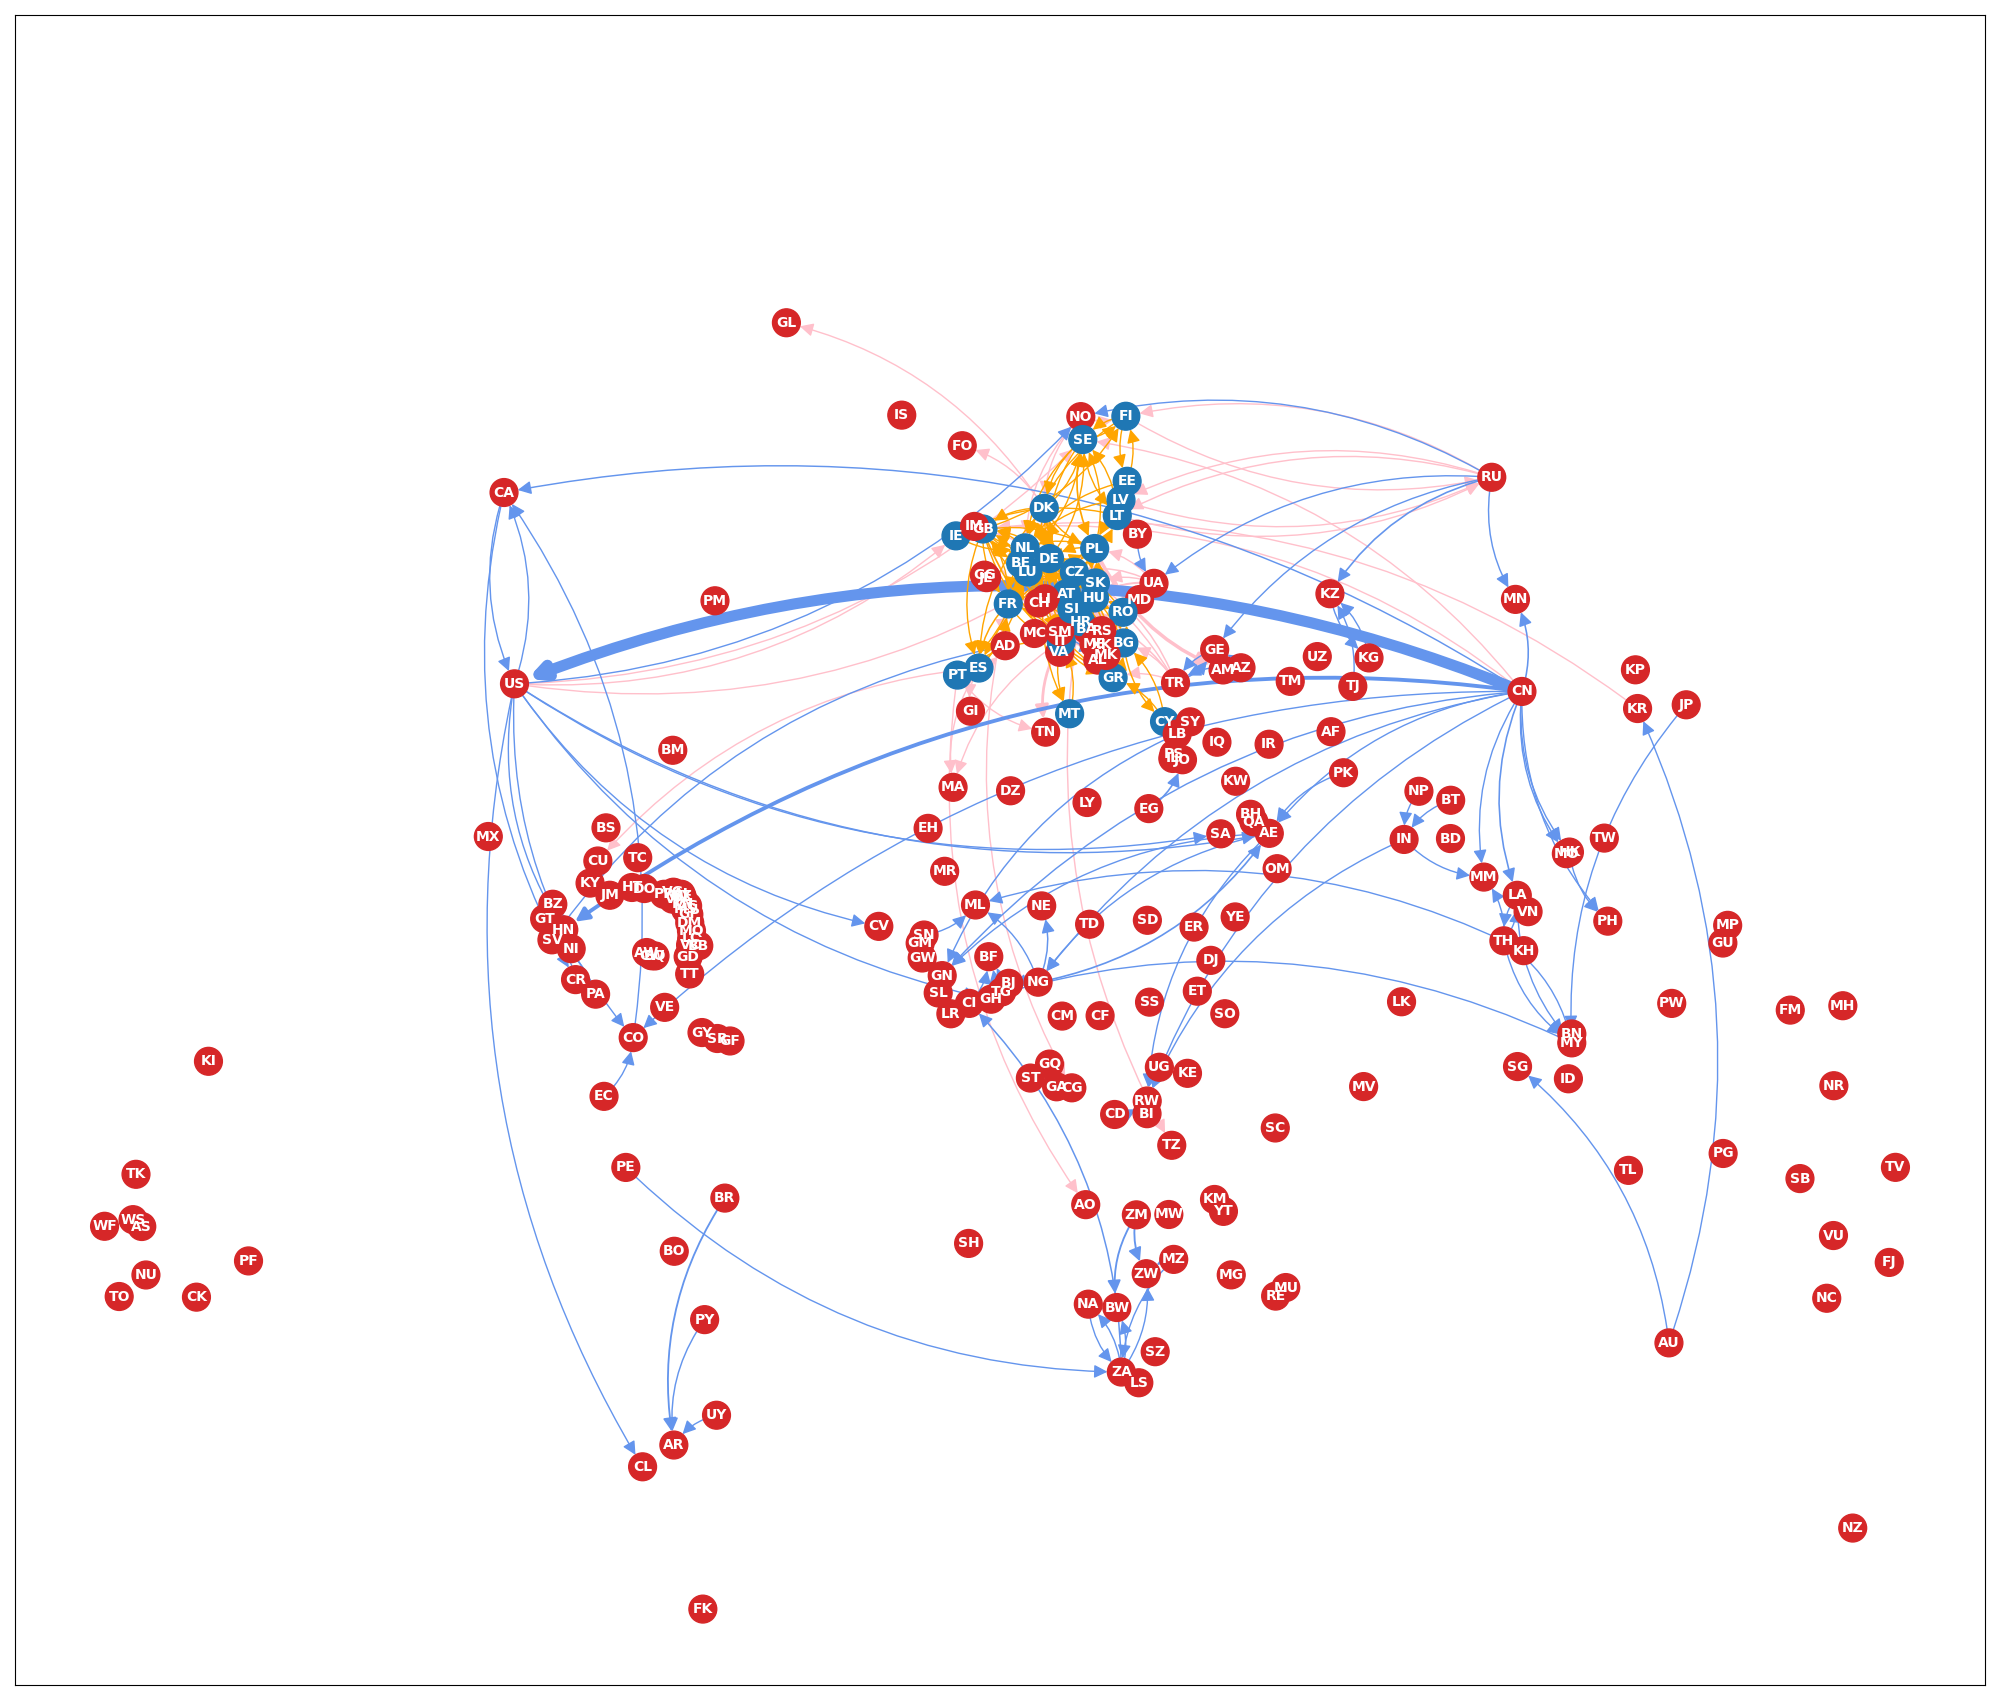
\includegraphics[height=0.4\textheight]{pics/full_y19_p35_force_79.png}
    \caption[Trade network for \textit{Electricity, gas, steam and air conditioning} in 2019]{Trade network for \textit{Electricity, gas, steam and air conditioning} in 2019, with countries located according to their geographical position.}
    \label{fig:elecgeo}
\end{figure}

\begin{figure}[H]
\centering
    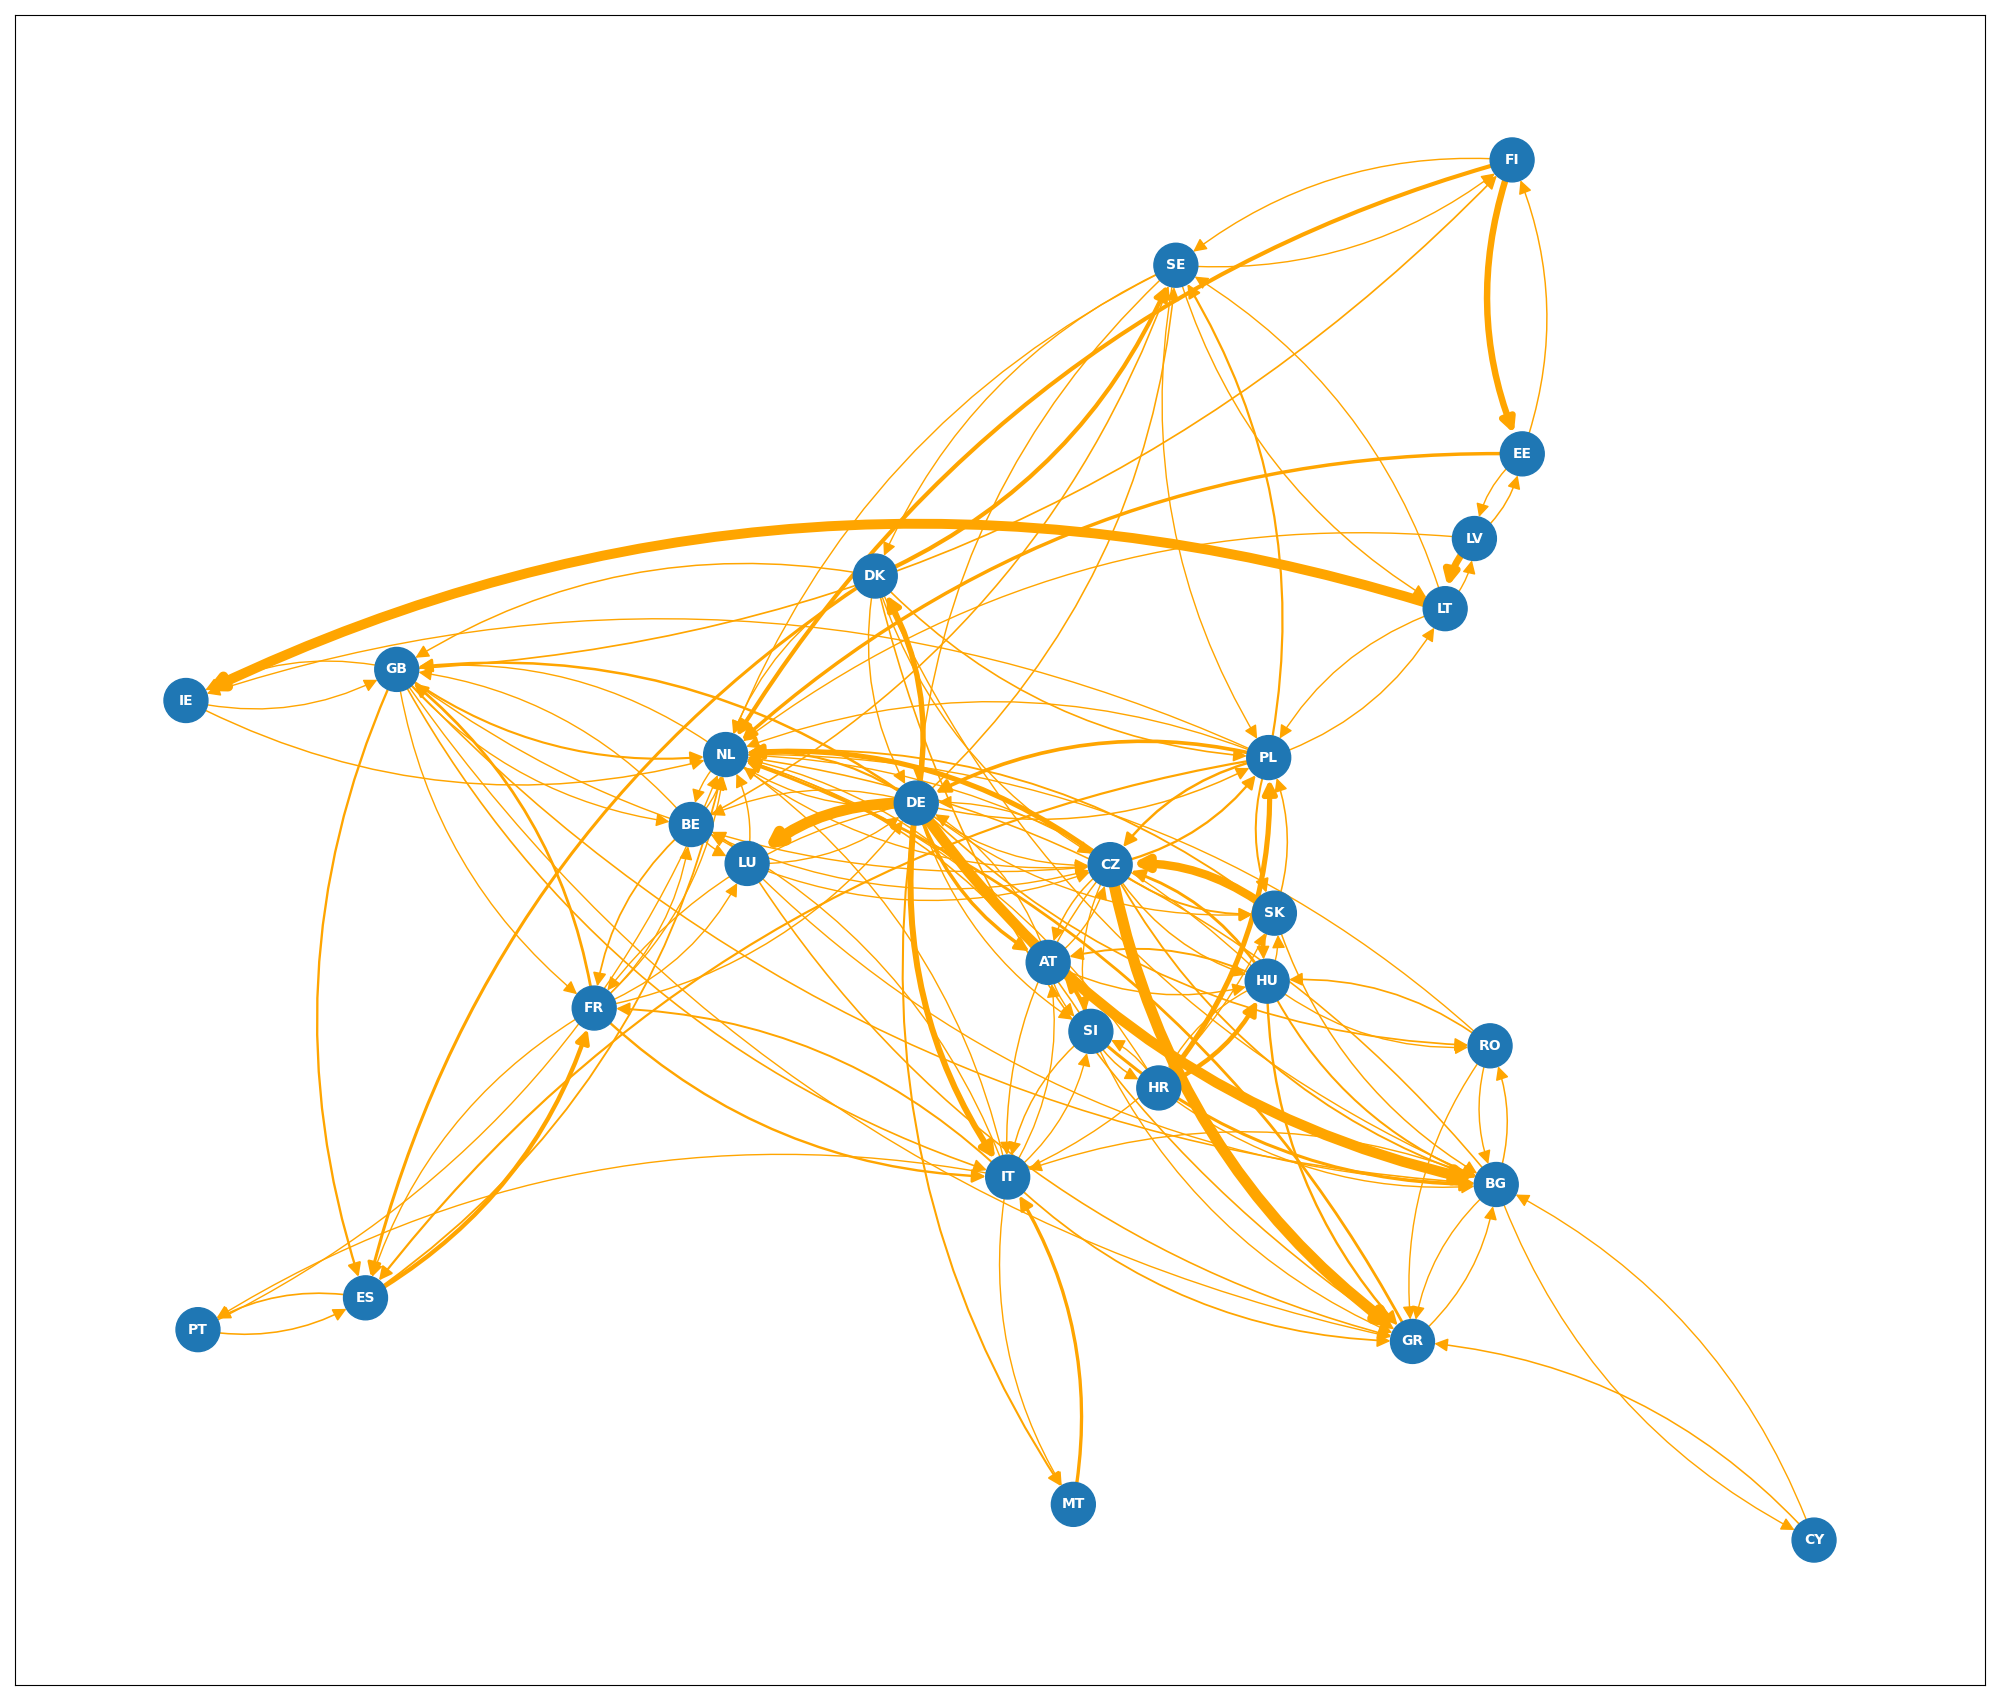
\includegraphics[height=0.4\textheight]{pics/full_y19_p35_force_82.png}
    \caption[Trade network for \textit{Electricity, gas, steam and air conditioning} in 2019 among European countries only.]{Trade network for \textit{Electricity, gas, steam and air conditioning} in 2019 among European countries only, with countries located according to their geographical position.}
    \label{fig:elecgeoeur}
\end{figure}
         

\section{The \textit{Food Products} Trade Network}

% - Food network abbastanza interessante perchè aveva size grossa, facilmente interpretabile
The market of \textit{Food Products} is particularly interesting since it is one of the biggest in terms of amount of money spent, and also its relationships may be easier to interpret. Global food trade is of crucial importance for countries since it guarantees food security and availability. Focusing on this category, it is possible to look at the graph metrics and how they evolve over time, which gives us a first impression of the dynamics of this network. In Figure \ref{fig:foodmetrics}, four metrics are shown as time series, displaying trends and variations due to the latest historical events. The chosen metrics are size (sum of the weights), average degree, median page rank and average clustering coefficient.

\begin{figure}
    \centering
    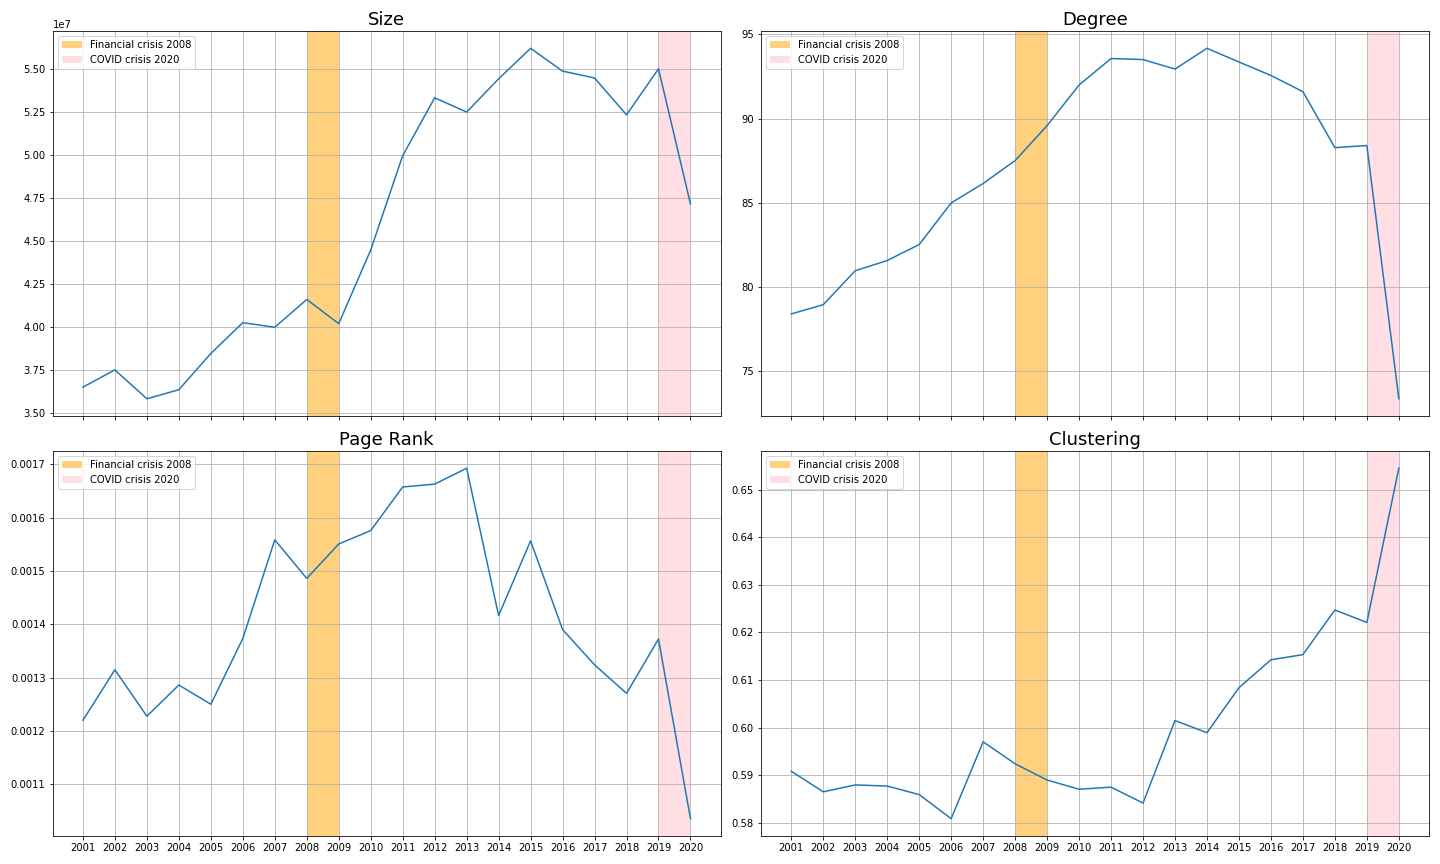
\includegraphics[width=\textwidth]{tex/pics/full_p10_metric_ts.png}
    \caption{Food Metrics}
    \label{fig:foodmetrics}
\end{figure}

In the upper left box, we can easily spot the effects of the 2008 financial crisis and the COVID crisis on the size of the graph. 
% From one year to the next, the amount of trade dropped by more than 10 million euros (per 1000 p.), and it even halved in 2020 with respect to 2019. 
Regarding 2020, we can see in the two plots on the right the effect of closing the borders to contain the pandemic: the average degree had a huge drop since countries truncated or reduced a significant number of exchanges. The steep increase in clustering instead can be attributed to it being inversely correlated with the average degree: when a node has fewer neighbors the denominator of Equation \ref{eq:clustering} decreases, and so the clustering coefficient goes up, even though the network as a whole may be less connected. 
Lastly, in the bottom right plot we see the median page rank among nodes, and we can observe that it used to have a positive trend until 2013, but since then it had started to go down, even more so during COVID. This could be a signal of the market going from a slightly more centralized structure to having more producers and exporters.

\begin{table}
    \centering
    \begin{tabular}{lrrrrr}
\toprule
Year & Sum of Weights & Mean Degree & Mean Weighted Degree & Mean Density & Mean Clustering Coef. \\
\midrule
2001 &   36509200.330 &      78.405 &           154047.259 &        0.166 &                 0.591 \\
2002 &   37513491.505 &      78.954 &           158284.774 &        0.167 &                 0.587 \\
2003 &   35834880.222 &      80.970 &           151202.026 &        0.172 &                 0.588 \\
2004 &   36360931.447 &      81.578 &           153421.652 &        0.173 &                 0.588 \\
2005 &   38465162.474 &      82.523 &           162300.264 &        0.175 &                 0.586 \\
2006 &   40252079.325 &      84.996 &           169839.997 &        0.180 &                 0.581 \\
2007 &   39986952.244 &      86.152 &           168721.317 &        0.183 &                 0.597 \\
2008 &   41599514.090 &      87.511 &           175525.376 &        0.185 &                 0.592 \\
2009 &   40194718.236 &      89.586 &           169597.967 &        0.190 &                 0.589 \\
2010 &   44470330.944 &      92.000 &           187638.527 &        0.195 &                 0.587 \\
2011 &   49944768.368 &      93.570 &           210737.419 &        0.198 &                 0.587 \\
2012 &   53301637.474 &      93.511 &           224901.424 &        0.198 &                 0.584 \\
2013 &   52476105.583 &      92.945 &           221418.167 &        0.197 &                 0.601 \\
2014 &   54403154.800 &      94.177 &           229549.176 &        0.200 &                 0.599 \\
2015 &   56174176.395 &      93.367 &           237021.841 &        0.198 &                 0.608 \\
2016 &   54850661.995 &      92.565 &           231437.392 &        0.196 &                 0.614 \\
2017 &   54454499.177 &      91.603 &           229765.819 &        0.194 &                 0.615 \\
2018 &   52311321.209 &      88.278 &           220722.874 &        0.187 &                 0.625 \\
2019 &   54985941.283 &      88.405 &           232008.191 &        0.187 &                 0.622 \\
2020 &   47139479.358 &      73.367 &           198900.757 &        0.155 &                 0.654 \\
\bottomrule
\end{tabular}

    \caption{Food Products Metrics}
    \label{tab:foodmetrics}
\end{table}

\paragraph{Degree distribution}






%     1) graph metrics: 
%         - over time
%         - power law over time
%     2) node properties:
%         - compared on average tra i nodi
%         - time series of relevant node's + pr
%     3) communities:
%         - grafico schschschschscsch (x2)
%         - plot confronto sbm vs louv 
%             --> fai vedere in cosa sono diversi (perchè le communities rappresentano cose diverse)
%             --> confronto modularities
%         - plot tanti^n plot





\section{The Gas and Energy Trade Network}
